\documentclass[conference]{IEEEtran}

\usepackage[utf8]{inputenc}
\usepackage[english]{babel}

\begin{document}

\title{Implementing 'Gordon': A NAO Robot Receptionist to Enhance Efficiency in Critical Services Using Choregraphe and Python}

\author{
\IEEEauthorblockN{
        Diana Milligan\IEEEauthorrefmark{1},
        Filip Hanuš\IEEEauthorrefmark{1},
        Harry Williams\IEEEauthorrefmark{1},\\
        Jack Thompson\IEEEauthorrefmark{1},
        Natalie Leung\IEEEauthorrefmark{1}
}
\IEEEauthorblockA{
        \IEEEauthorrefmark{1}School of Engineering, College of Art, Technology and Environment,\\ University of the West of England, Bristol, UK\\
        Email: \{diana2.milligan, filip2.hanus, harry4.williams, jack2.ould, wing7.leung\}@live.uwe.ac.uk}
}

\maketitle

\begin{abstract}

This paper presents what is in this abstract. 

\end{abstract}

\begin{IEEEkeywords}

NAO Robot, Human Robot Interaction.

\end{IEEEkeywords}

\section{Introduction}

The purpose of this project is to use a Nao robotic platform to effectively perform a task that requires direct interaction with human. 
There are many different metrics that can be used to quantify the success of such a system, but as a broader definition an effective system 
should be able to receive and convey relevant information to an untrained user to achieve a wider goal.

A task that lends itself to this project brief is a reception environment, particularly in a medical setting. According to 
(source), managerial staff shortages within the NHS has pushed clinical staff to spend more time on administrative task over 
patient-facing care. To effectively reduce staffing requirements and thus make the running of medical centres less resource intensive, robotic 
systems can be integrated to alleviate the bulk of repetitive tasks. A good low-risk opportunity for this kind of integration is within a 
receptionist role where any possible errors are of a significantly lower severity than other roles (e.g. medical diagnosis and treatment).
A study conducted by (source) tested the concept of a robotic receptionist for medical purposes, concluding that the robot displayed a 
"proffesional level of friendliness" that made it suited the role. However, the testing used a Wizard-of-Oz method with the robot only 
used as the interface between a user and a remote operator. Had all the behaviours been generated by the robot, there could have been 
a significant difference in how it was perceived by users.

Methods to create a sense of authority for robots has been explored through many different ways, many of which can be implemented within 
this project. (source) explored the effect of height on robotic telepresence systems, concluding that a shorter "leader" was less persuasive 
for a the human follower. As well as the robot's stature, (source) found that contextual information such as the location of an interaction 
helped users infer the robot’s role.

Appearance has been argued to be a less important factor by (source) who tested a variety of different variables for artificial agents, with an 
anthropomorphism and behaviour being " the most significant factors in predicting the trust and compliance with the robot" rather 
than physical appearance. A Nao platform has been used by (source) to test the limitations of such compliance, finding that users would 
refuse to follow challenging orders from a robot if factors such as perceived intelligence or professionalism were compromised.


\section{Literature Review}

TBD

\section{Design and Methodology}

The system design for our NAO robot receptionist was guided by two goals: providing a seamless user experience and supporting medical
staff through reliable automated interactions. Drawing on Sutherland et al.’s work \cite{Sutherland2019}, which established the feasibility of a
medical robot receptionist, we sought to move beyond Wizard-of-Oz methods by having NAO autonomously recognise faces, detect gestures, and facilitate 
patient check-in. Additionally, evidence from Rae et al. \cite{Rae2013} encouraged us to position the robot at a height that aligns with typical eye 
level, increasing the robot’s perceived authority and engagement. Key interaction modes include speech (British English), gesture recognition, and 
email alerts, which were selected to replicate the essential tasks usually performed by human receptionists.

\begin{figure*}
        \centering
        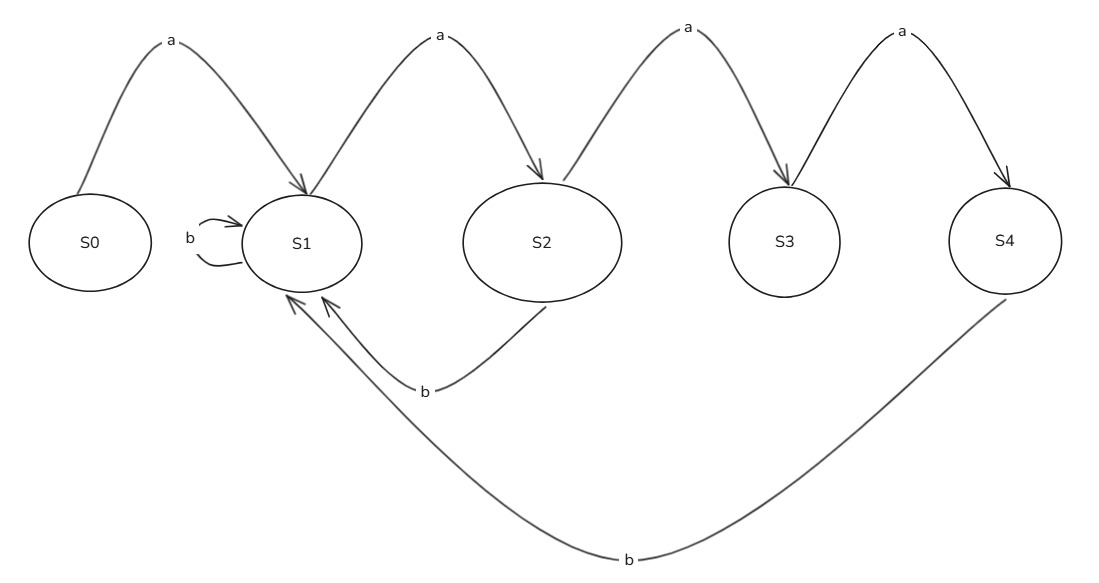
\includegraphics[width=.6\linewidth]{states.jpg}
        \caption{Different States and their Connections}
        \label{Different states}
\end{figure*}

As shown in the figure~\ref{Different states}, our approach centred on a modular pipeline, implemented using Aldebaran’s Choregraphe software and Python-based scripts. 
First, the robot engages 
in face detection (State 0), aided by an external camera if necessary. Should an individual approach or wave (State 1), detected via Mediapipe Python script,
the system transitions to a conversation phase (State 2), where NAO uses inbuilt speech recognition to guide the patient through check-in queries.
To confirm arrival, an email is automatically sent to the relevant staff member (State 3), ensuring prompt notification. 
Finally, a simple feedback process (State 4) invites users to rate their experience with the robot, capturing qualitative data for further improvements.
This staged flow was developed to make sure that, at each step, NAO’s actions could be isolated and tested independently before being integrated into
the overall receptionist framework. Due to potential connectivity restrictions, such as network blocks on Simple Mail Transfer Protocol (SMTP), contingency 
plans were introduced. In alignment with findings by Bistolfi \cite{Bistolfi2022}, allowing for quick human intervention in case of failure was essential 
to maintain trust and minimise disruptions. By structuring each component in a self-contained manner, we aimed to achieve higher system reliability, 
mitigate user frustration, and conform to healthcare settings where uninterrupted service is imperative.


\section{Testing and Results}

TBD

\section{Future Work}

TBD

\section{Conclusion}

TBD

\bibliographystyle{plain}
\bibliography{references}

\end{document}